%%%%%%%%%%%%%%%%%%%%%%%%%%%%%%%%%%%%%%%%%%%%%%%%
% Template TCMN data sheet version 3
% 
% Alberto Sanchez asanchezrodelgo@ifc.org Dec 2015
%%%%%%%%%%%%%%%%%%%%%%%%%%%%%%%%%%%%%%%%%%%%%%%%
\documentclass{article}\usepackage[]{graphicx}\usepackage[]{color}
%% maxwidth is the original width if it is less than linewidth
%% otherwise use linewidth (to make sure the graphics do not exceed the margin)
\makeatletter
\def\maxwidth{ %
  \ifdim\Gin@nat@width>\linewidth
    \linewidth
  \else
    \Gin@nat@width
  \fi
}
\makeatother

\definecolor{fgcolor}{rgb}{0.345, 0.345, 0.345}
\newcommand{\hlnum}[1]{\textcolor[rgb]{0.686,0.059,0.569}{#1}}%
\newcommand{\hlstr}[1]{\textcolor[rgb]{0.192,0.494,0.8}{#1}}%
\newcommand{\hlcom}[1]{\textcolor[rgb]{0.678,0.584,0.686}{\textit{#1}}}%
\newcommand{\hlopt}[1]{\textcolor[rgb]{0,0,0}{#1}}%
\newcommand{\hlstd}[1]{\textcolor[rgb]{0.345,0.345,0.345}{#1}}%
\newcommand{\hlkwa}[1]{\textcolor[rgb]{0.161,0.373,0.58}{\textbf{#1}}}%
\newcommand{\hlkwb}[1]{\textcolor[rgb]{0.69,0.353,0.396}{#1}}%
\newcommand{\hlkwc}[1]{\textcolor[rgb]{0.333,0.667,0.333}{#1}}%
\newcommand{\hlkwd}[1]{\textcolor[rgb]{0.737,0.353,0.396}{\textbf{#1}}}%

\usepackage{framed}
\makeatletter
\newenvironment{kframe}{%
 \def\at@end@of@kframe{}%
 \ifinner\ifhmode%
  \def\at@end@of@kframe{\end{minipage}}%
  \begin{minipage}{\columnwidth}%
 \fi\fi%
 \def\FrameCommand##1{\hskip\@totalleftmargin \hskip-\fboxsep
 \colorbox{shadecolor}{##1}\hskip-\fboxsep
     % There is no \\@totalrightmargin, so:
     \hskip-\linewidth \hskip-\@totalleftmargin \hskip\columnwidth}%
 \MakeFramed {\advance\hsize-\width
   \@totalleftmargin\z@ \linewidth\hsize
   \@setminipage}}%
 {\par\unskip\endMakeFramed%
 \at@end@of@kframe}
\makeatother

\definecolor{shadecolor}{rgb}{.97, .97, .97}
\definecolor{messagecolor}{rgb}{0, 0, 0}
\definecolor{warningcolor}{rgb}{1, 0, 1}
\definecolor{errorcolor}{rgb}{1, 0, 0}
\newenvironment{knitrout}{}{} % an empty environment to be redefined in TeX

\usepackage{alltt}
%%%%%%%%%%%%%% package declaration %%%%%%%%%%%%%%%%%%%%%
\usepackage[top=0.3in, bottom=0.1in, left=0.5in, right=0.6in]{geometry}
\usepackage{graphicx} % to load images
\usepackage[export]{adjustbox} % add alignment to includegraphics
\usepackage[font=small]{caption}
\usepackage{xcolor} % color text
\usepackage{tabularx} % to adjust table width, etc. 
\usepackage{titlesec} % format titles and headers
\usepackage{sectsty} % format sections & subsections
\usepackage{booktabs} % For \toprule, \midrule and \bottomrule
\usepackage[colorlinks = true,
            linkcolor = blue,
            urlcolor  = blue,
            citecolor = blue,
            anchorcolor = blue]{hyperref} % to include hyperlinks in the doc
\sectionfont{\fontsize{16}{15}\selectfont\raggedright} % formats title newsletter (section) 
\subsectionfont{\fontsize{14}{12}\selectfont\raggedright} % formats title newsletter (section)
%%%%%%%%%%%%%%%%%%%%%%%%%%%%%%%%%%%%%%%%%%%%%%%%%%%%%%%%%%%%%%%%%%%%%%%%%%%%%%%%%%%
%
%%%%%%%%%%%%%%%%%%%%%%%%%%%%%%%%%%%%% BEGIN DOCUMENT %%%%%%%%%%%%%%%%%%%%%%%%%%%%%%
\IfFileExists{upquote.sty}{\usepackage{upquote}}{}
\begin{document}

%

%%%%%%%%%%%%%%%% PAGE 1 %%%%%%%%%%%%%%%%%%%
%World Bank logo and TCMN branding
\begin{figure}
  \vspace{-3ex} % move up this figure
  \hspace{-7ex} % move left this figure
  \includegraphics[width=5cm]{/Users/asanchez3/shinyTCMN/www/wb_logo_background.png}
\end{figure}
\begin{figure}
  \begin{minipage}[t]{0.99\textwidth} % top section
      \vspace{-30ex}
      \hspace{-2ex}
      \raggedright{\includegraphics[width=5.5cm,right]{/Users/asanchez3/shinyTCMN/www/TC_snapshots_data.png}}
  %  {\color{white!70!black}\noindent\makebox[\linewidth]{\rule{20cm}{0.3pt}}} % horiz line
  \end{minipage}
\end{figure}
%
%%%% Macro Indicators
\begin{minipage}[t]{0.99\textwidth} % top section
  \vspace{-1.5cm}
  \begin{minipage}[c]{0.36\textwidth} 
    \begin{minipage}[c]{0.28\textwidth} % flag
      \includegraphics[width=1.2cm,height=1.2cm]{/Users/asanchez3/shinyTCMN/www/CN.png}
    \end{minipage}
    \begin{minipage}[c]{0.70\textwidth} % Country name
      \section*{\color{blue!40!black}China}
    \end{minipage}
  \end{minipage}
  \begin{minipage}[c]{0.63\textwidth} % key macro table 
    % Table 1
    \centering
    \resizebox{\textwidth}{!}{
% latex table generated in R 3.2.2 by xtable 1.7-4 package
% Wed Feb 17 09:01:52 2016
{\LARGE
\begin{tabular}{>{\centering}p{1.5in}>{\centering}p{1.5in}>{\centering}p{1.5in}>{\centering}p{1.5in}>{\centering}p{1.5in}>{\centering}p{1.5in}>{\centering}p{1.5in}l}
  GDP (US\$ billions) (2016) & Population (millions) (2016) & Income per capita (current US\$) (2016) & Poverty rate (2010) & Unemployment rate (2014) &  &  &  \\ 
  11,655.6 &  1,378.2 &  8,456.9 &     11.2 &      4.7 &  &  &  \\ 
  \end{tabular}
}

    }
  \end{minipage}  
\end{minipage} % end top section

\begin{minipage}[b]{0.99\textwidth} % macro indicators main table
  %\vspace*{0.5cm}
  %\vspace{+3ex}
  \begin{minipage}[t]{0.99\textwidth}
%'     \begin{minipage}[c]{0.875\textwidth}
%'       \begin{flushleft}  
%'       {\color{blue!50!black} \textbf{\small Macro Indicators}}
%'       \end{flushleft} 
%'       \vspace*{-0.4cm}
%'       % Table 2
%'       \centering
%'       \resizebox{\textwidth}{!}{
%'     <<macroInd_Big,echo=FALSE,message=FALSE,cache=FALSE,warning=FALSE,fig.align='center',results="asis">>=  
%'       @      
%'       }
%'       \end{minipage}
%'       \begin{minipage}[c]{0.12\textwidth}
%'       \vspace*{+0.9cm}
%'           <<createSparklines,echo=FALSE,message=FALSE,cache=FALSE,warning=FALSE,fig.align='center',fig.height=11,fig.width=4,results="asis">>=  
%'       @
%'       \vspace*{-0.4cm}
%'       \end{minipage}
 
    \begin{minipage}[c]{0.875\textwidth}
      \begin{flushleft}  
      {\color{white!30!blue} \textbf{\small Macro Indicators}}
      \end{flushleft} 
      \vspace*{-0.4cm}
      % Table 2
      \centering
      \resizebox{\textwidth}{!}{
% latex table generated in R 3.2.2 by xtable 1.7-4 package
% Wed Feb 17 09:01:52 2016
{\Large
\begin{tabular}{>{\raggedright}p{6in}r>{\raggedleft}p{0.8in}>{\raggedleft}p{0.8in}>{\raggedleft}p{0.8in}>{\raggedleft}p{0.8in}>{\raggedleft}p{0.8in}l}
  & Avg 2002-2011 & 2012 & 2013 & 2014 & 2015 & 2016 &  \\ 
  \hline
GDP growth (annual \%) &  10.39 &   7.70 &   7.70 &   7.30 &   6.95 &   6.70 &  \\ 
  Current account balance &   4.72 &   2.61 &   2.23 &   2.53 &   3.55 &   3.94 &  \\ 
  Fiscal balance (\% of GDP) &  -1.44 &   0.02 &  -1.14 &  -1.94 &  -2.82 &  -1.87 &  \\ 
  Remittances, received (\% of GDP) \large{[1]} &   0.36 &   0.20 &   0.19 &   0.29 & --- & --- &  \\ 
  Real Effective Exchange Rate (2010=100) &  89.34 & 113.94 & 121.36 & 124.76 & 133.39 & 131.69 &  \\ 
  Consumer Price Index, annual percent change &   2.47 &   2.60 &   2.58 &   2.06 &   1.32 &   1.32 &  \\ 
  \end{tabular}
}

      }
    \end{minipage}
    \begin{minipage}[c]{0.11\textwidth}
      \vspace*{+0.8cm}


{\centering 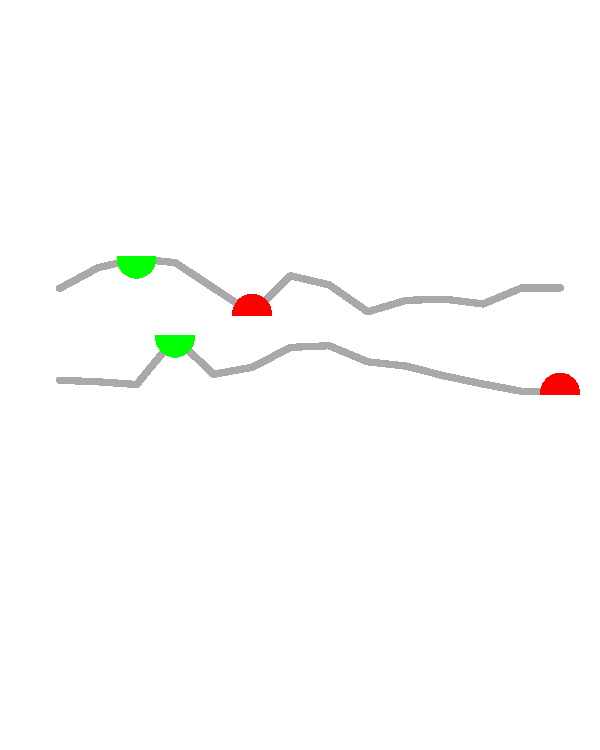
\includegraphics[width=\maxwidth]{figure/createSparklines_macro-1} 

}



      \vspace*{-0.5cm}
    \end{minipage}
    
    %\vspace*{-0.4cm}
    \begin{minipage}[c]{0.875\textwidth}
      \begin{flushleft}  
      {\color{white!30!blue} \textbf{\small Investment indicators}}
      \end{flushleft} 
      \vspace*{-0.4cm}
      % Table 2
      \centering
      \resizebox{\textwidth}{!}{
% latex table generated in R 3.2.2 by xtable 1.7-4 package
% Wed Feb 17 09:01:52 2016
{\Large
\begin{tabular}{>{\raggedright}p{6in}r>{\raggedleft}p{0.8in}>{\raggedleft}p{0.8in}>{\raggedleft}p{0.8in}>{\raggedleft}p{0.8in}>{\raggedleft}p{0.8in}l}
  & Avg 2002-2011 & 2012 & 2013 & 2014 & 2015 & 2016 &  \\ 
  \hline
Gross domestic investment (\% GDP) & 38.9 & 44.6 & 44.7 & 44.5 & 43.9 & 43.2 &  \\ 
  Gross domestic investment, of w: Private investment (\% GDP) \large{[1]} & 44.0 & 47.3 & 47.7 & 46.2 & --- & --- &  \\ 
  Inward FDI (\% of GDP) \large{[2]} &  2.6 &  1.5 &  1.3 &  1.3 & --- & --- &  \\ 
  Inward FDI, \% of private investment \large{[2]} &  6.5 &  3.1 &   NA & --- & --- & --- &  \\ 
  \end{tabular}
}

      }
    \end{minipage}
    \begin{minipage}[c]{0.11\textwidth}
      \vspace*{+0.8cm}


{\centering 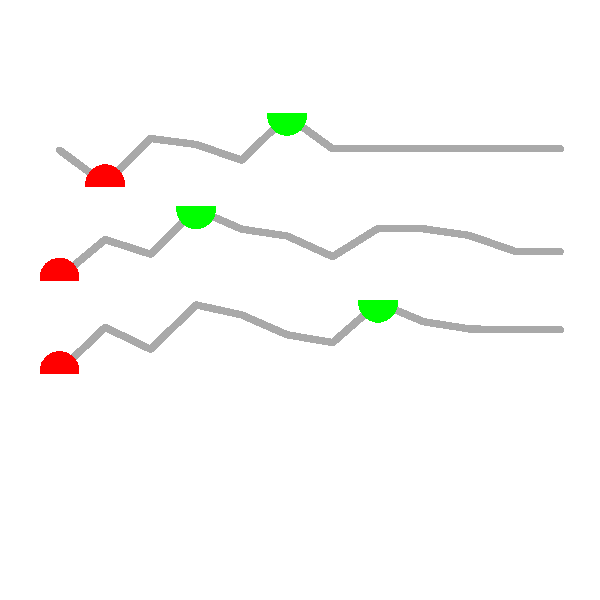
\includegraphics[width=\maxwidth]{figure/createSparklines_invest-1} 

}



      \vspace*{-0.5cm}
    \end{minipage}
    
    %\vspace*{-0.4cm}
    \begin{minipage}[c]{0.875\textwidth}
      \begin{flushleft}  
      {\color{white!30!blue} \textbf{\small Trade Indicators}}
      \end{flushleft} 
      \vspace*{-0.4cm}
      % Table 2
      \centering
      \resizebox{\textwidth}{!}{
% latex table generated in R 3.2.2 by xtable 1.7-4 package
% Wed Feb 17 09:01:53 2016
{\Large
\begin{tabular}{>{\raggedright}p{6in}r>{\raggedleft}p{0.8in}>{\raggedleft}p{0.8in}>{\raggedleft}p{0.8in}>{\raggedleft}p{0.8in}>{\raggedleft}p{0.8in}l}
  & Avg 2002-2011 & 2012 & 2013 & 2014 & 2015 & 2016 &  \\ 
  \hline
Total Trade in Goods and Services (\% of GDP, real terms) & 60.7 & 65.9 & 65.5 & 64.8 & 63.6 & 62.4 &  \\ 
  Trade balance (\% GDP, real terms) &  4.5 &  5.6 &  5.5 &  5.6 &  5.8 &  5.9 &  \\ 
  Exports, Goods and Services, annual percent change (real terms) & 15.6 &  3.9 &  6.9 &  6.5 &  5.4 &  5.0 &  \\ 
  Imports, Goods and Services, annual percent change (real terms) & 14.5 &  5.2 &  7.2 &  5.9 &  4.5 &  4.2 &  \\ 
  Total reserves in months of imports \large{[1]} & 19.1 & 19.0 & 19.8 & --- & --- & --- &  \\ 
  \end{tabular}
}

      }
    \end{minipage}
    \begin{minipage}[c]{0.11\textwidth}
      \vspace*{+0.8cm}


{\centering 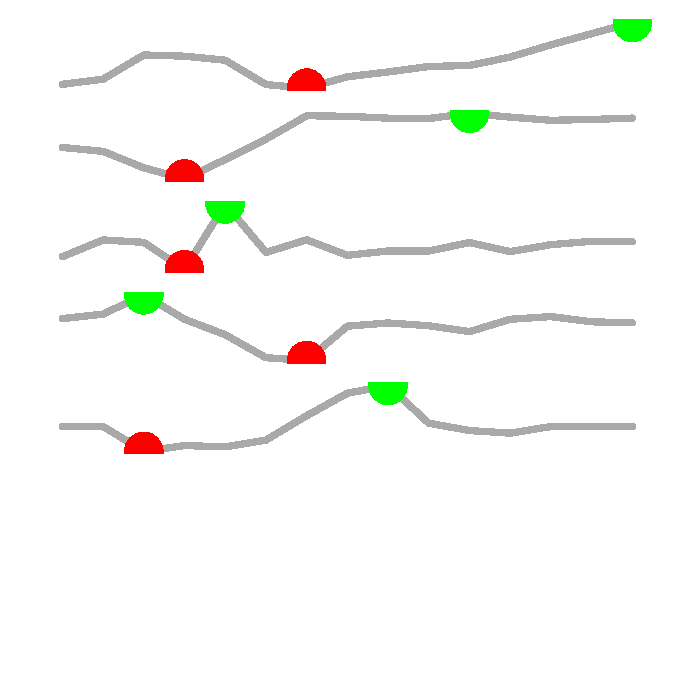
\includegraphics[width=\maxwidth]{figure/createSparklines_trade-1} 

}



      \vspace*{-0.4cm}
    \end{minipage}
  \\[3pt]
\raggedright{\footnotesize{\href{http://www.worldbank.org/en/topic/macroeconomics/overview}{Sources: MFM note}{,} \href{http://data.worldbank.org/data-catalog/world-development indicators}{[1] World Development Indicators (WDI)}{,} \href{http://unctadstat.unctad.org/wds/ReportFolders/reportFolders.aspx}{[2] UNCTADSTAT}{,} \href{https://www.imf.org/external/pubs/ft/weo/2015/02/weodata/index.aspx}{[3] World Economic Outlook (WEO)}}}
  \end{minipage} 
%\end{minipage}    
  \begin{minipage}[b]{\textwidth} % macro charts
  \vspace{+3ex}
    \begin{minipage}[c]{0.49\textwidth} % imports/exports 
    \center{\color{blue!50!black} \textbf{\small Goods Export and Import \\ volume growth, 2012-2015}}


{\centering 
\includegraphics[width=\maxwidth]{figure/ExpImp_HF-1} 

}



    \vspace*{-0.3cm}
    %\hspace*{0.5cm} 
    \raggedright{\footnotesize{\href{http://web.worldbank.org/WBSITE/EXTERNAL/EXTDEC/EXTDECPROSPECTS/0,,menuPK:476941~pagePK:51084723~piPK:51084722~theSitePK:476883,00.html}{Source: Development Prospects Group (DECPG)}}}
    \end{minipage}
    \begin{minipage}[c]{0.49\textwidth} % gdp value added
    \center{\color{blue!50!black} \textbf{\small Gross Value Added by \\ Economic Activity 2013 \footnotesize(\% GDP)}}


{\centering 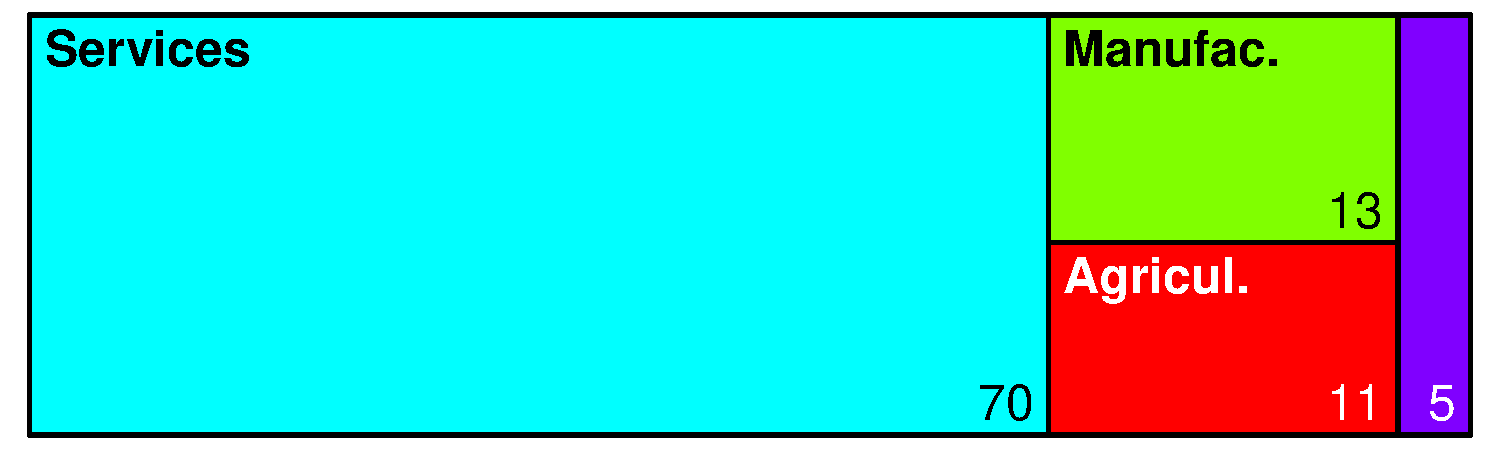
\includegraphics[width=\maxwidth]{figure/GVA_Treemap-1} 

}



   %\vspace*{-0.3cm}
   %\hspace*{0.5cm} 
   \raggedright{\footnotesize{\href{http://data.worldbank.org/data-catalog/world-development indicators}{Source: World Development Indicators (WDI)}}}
    \end{minipage}
  \end{minipage}  
\end{minipage}   
 
%%%% Exports Imports and DB
\begin{minipage}[b]{0.99\textwidth}
  \vspace{0.8cm}
   \begin{minipage}[c]{0.44\textwidth} 
    %\vspace*{-0.2cm}
    \begin{minipage}[t]{0.99\textwidth} 
      {\color{blue!50!black} \textbf{\small Top 5 Exports by \% of Total Value, 2014}}
      %\vspace{3ex}
      \\[6pt]
      \centering
      \resizebox{\textwidth}{!}{%


{\centering 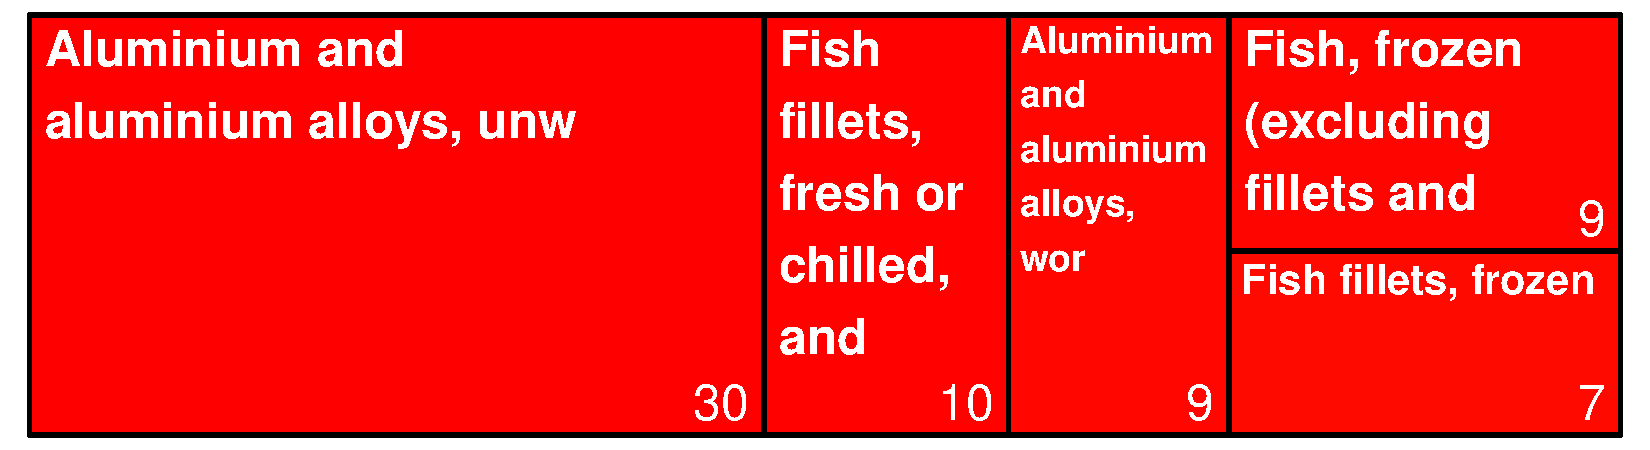
\includegraphics[width=\maxwidth]{figure/ImpExp_Treemap-2-1} 

}



      }
      \end{minipage}
      \\[14pt]
      \begin{minipage}[t]{0.99\textwidth} 
      {\color{blue!50!black} \textbf{\small Imports Categories by \% of Total Value, 2014}}
      \\[6pt]
      \centering
      \resizebox{\textwidth}{!}{%


{\centering 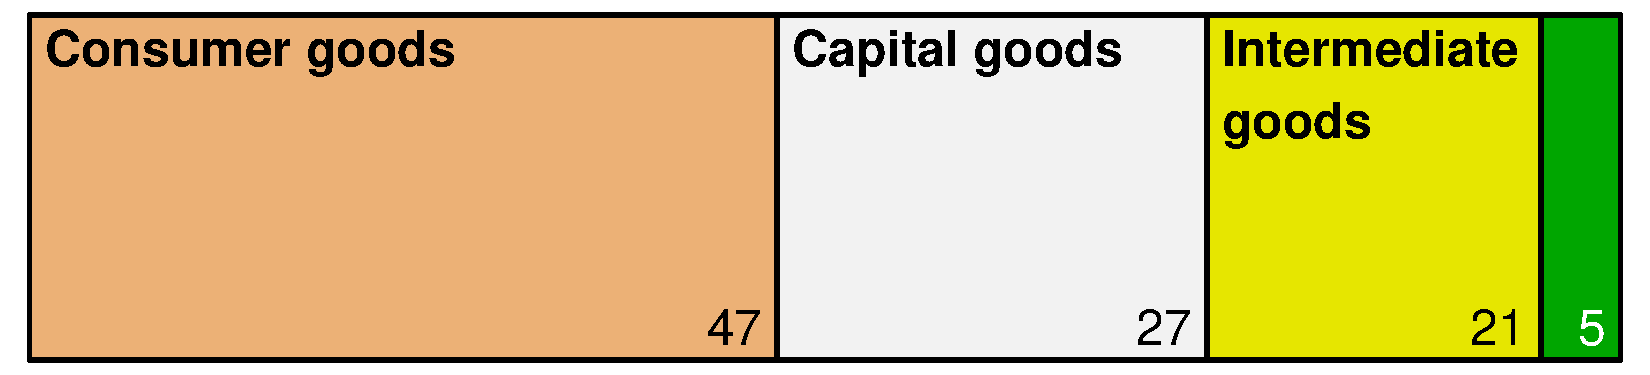
\includegraphics[width=\maxwidth]{figure/ImpExp_Treemap-1-1} 

}



      }
      \end{minipage}
      \\[10pt]
    %\hspace*{0.5cm}
    \footnotesize{\href{http://wits.worldbank.org}{Source: World Integrated Trade Solution (WITS)}} 
    \end{minipage}
    \begin{minipage}[c]{0.56\textwidth} % Doing Business table
    %\vspace*{-0.1cm}
    %\begin{flushleft}
      \center {\color{blue!50!black}\textbf{\small Doing Business 2015 Ranks \\ \footnotesize (among all countries)}}
    %\end{flushleft}
    \\[18pt]
    \centering
      \resizebox{\textwidth}{!}{%
% latex table generated in R 3.2.2 by xtable 1.7-4 package
% Wed Feb 17 09:01:54 2016
{\large
\begin{tabular}{lrrrr}
  & DB 2015 Rank & DB 2016 Rank & Change in Rank &  \\ 
  \hline
Dealing with Construction Permits & 177 & 176 & \color{green}{\Large1} &  \\ 
  Ease of Doing Business Rank & 83 & 84 & \color{red}{\Large-1} &  \\ 
  Enforcing Contracts & 7 & 7 & 0 &  \\ 
  Getting Credit & 71 & 79 & \color{red}{\Large-8} &  \\ 
  Getting Electricity & 86 & 92 & \color{red}{\Large-6} &  \\ 
  Paying Taxes & 133 & 132 & \color{green}{\Large1} &  \\ 
  Protecting Minority Investors & 133 & 134 & \color{red}{\Large-1} &  \\ 
  Registering Property & 41 & 43 & \color{red}{\Large-2} &  \\ 
  Resolving Insolvency & 53 & 55 & \color{red}{\Large-2} &  \\ 
  Starting a Business & 127 & 136 & \color{red}{\Large-9} &  \\ 
  Trading Across Borders & 96 & 96 & 0 &  \\ 
  \end{tabular}
}

      }
    \\[28pt]
     %\hspace*{0.5cm} 
     \raggedright{\footnotesize{\href{http://www.doingbusiness.org/data}{Source: Doing Busines Report 2015}}}
    \end{minipage}
\end{minipage}

% \vspace{+3ex}
% {\color{blue!50!white}\noindent\makebox[\linewidth]{\rule{18cm}{0.3pt}}} % horiz line
% \begin{minipage}[c]{0.99\textwidth}
%   \hspace*{-0.4cm}\raggedleft{\color{white!40!black} \footnotesize TRADE AND COMPETITIVENESS MONITORING NOTE - UPDATED} 
%   %month year}
% \end{minipage}

\newpage
%%%%%%%%%%%%%%%% PAGE 2 %%%%%%%%%%%%%%%%%%%

\begin{minipage}[t]{0.99\textwidth}
  \vspace{0.5cm}
  \begin{minipage}[c]{0.48\textwidth} % WEF Radar
    \center{\color{blue!50!black} \textbf{WEF Competitiveness Indicators \\ \footnotesize(Scale 1-5, 5=best)}}
    \vspace*{-0.6cm}


{\centering 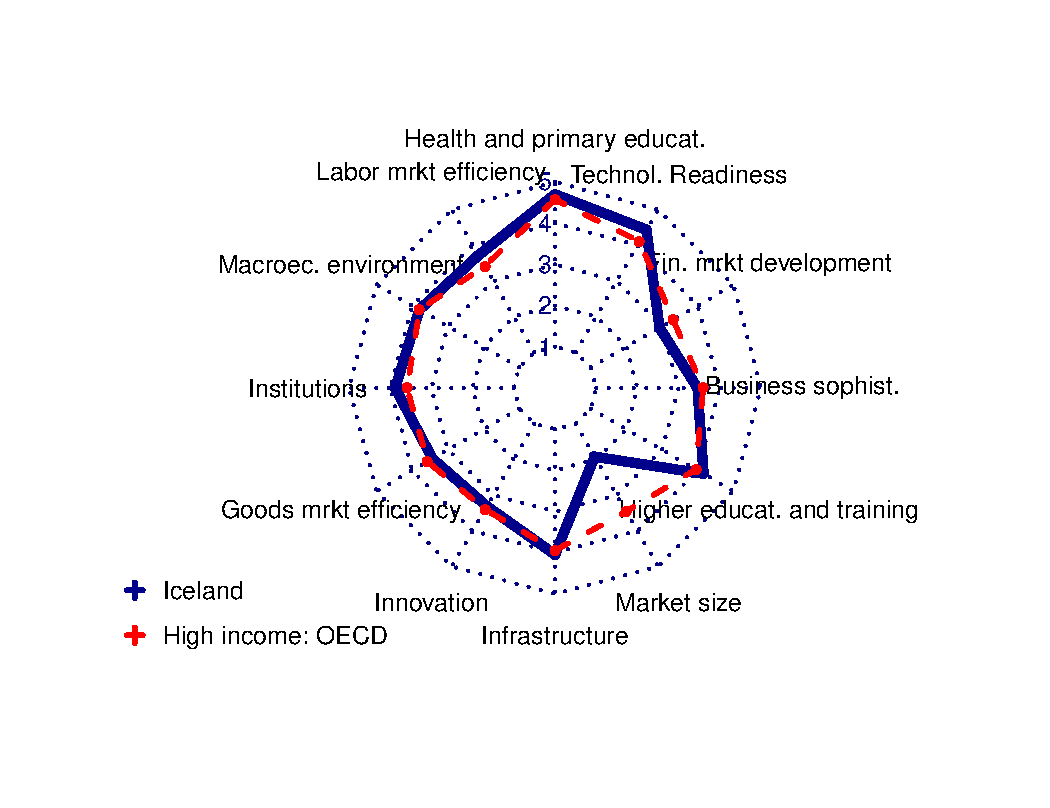
\includegraphics[width=\maxwidth]{figure/WEFradar-1} 

}



    \vspace*{-1.2cm} 
    \hspace*{0.3cm} \raggedright\footnotesize{\href{http://www.weforum.org/reports/global-competitiveness-report-2015-2016}{Source: WEF Global Competitiveness Report 2015}}
  \end{minipage}
  \begin{minipage}[c]{0.50\textwidth} % LPI chart
  %\vspace*{0.5cm}
  \center {\color{blue!50!black} \textbf{Logistics Performance Index \\ \footnotesize(Scale 1-5, 5=best)}}
    \vspace*{0.4cm}


{\centering 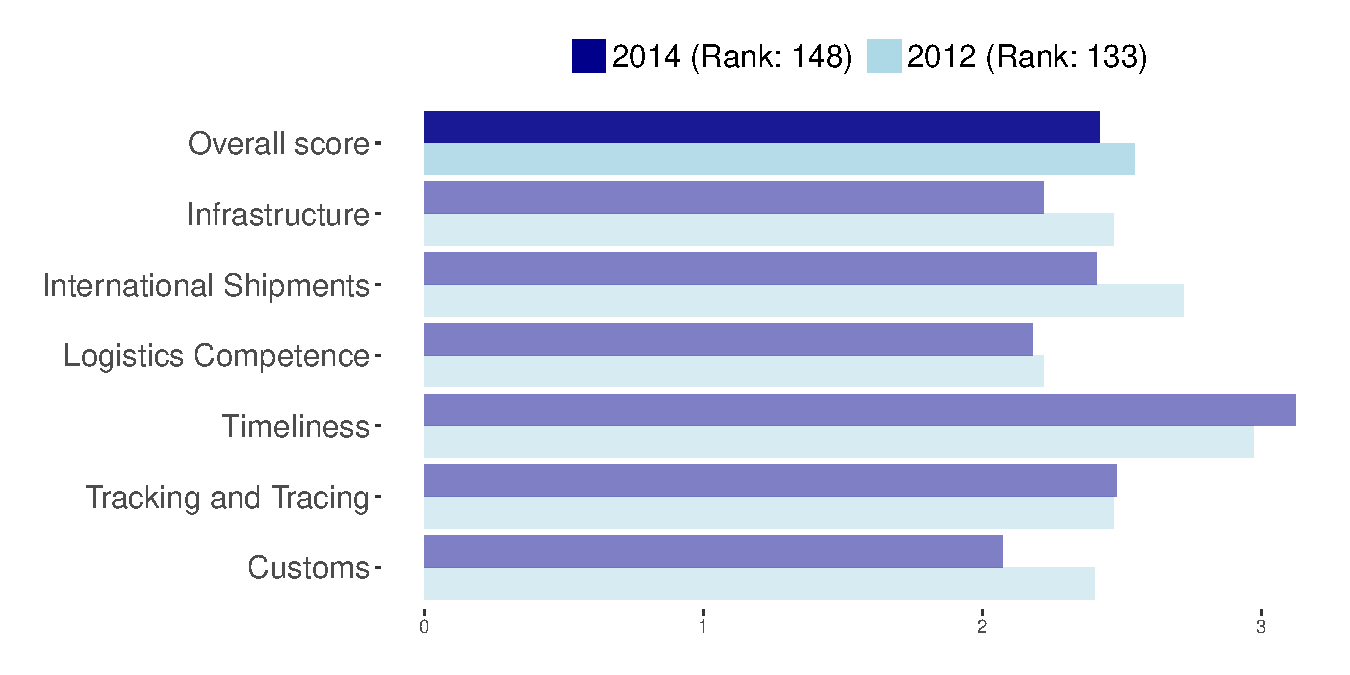
\includegraphics[width=\maxwidth]{figure/LPIindicators-1} 

}



  %\hspace*{0.5cm} 
  \raggedright\footnotesize{\href{http://lpi.worldbank.org}{Source: Logistics Performance Index (World Bank)}}
  \end{minipage}
\end{minipage}  

\begin{minipage}[b]{0.99\textwidth}
  \begin{minipage}[c]{0.50\textwidth} % WGI chart
    \vspace*{0.8cm}
    \center {\color{blue!50!black} \textbf{World Governance indicators \\ \footnotesize(Std. score, High=best)}}
    \vspace*{0.3cm}


{\centering 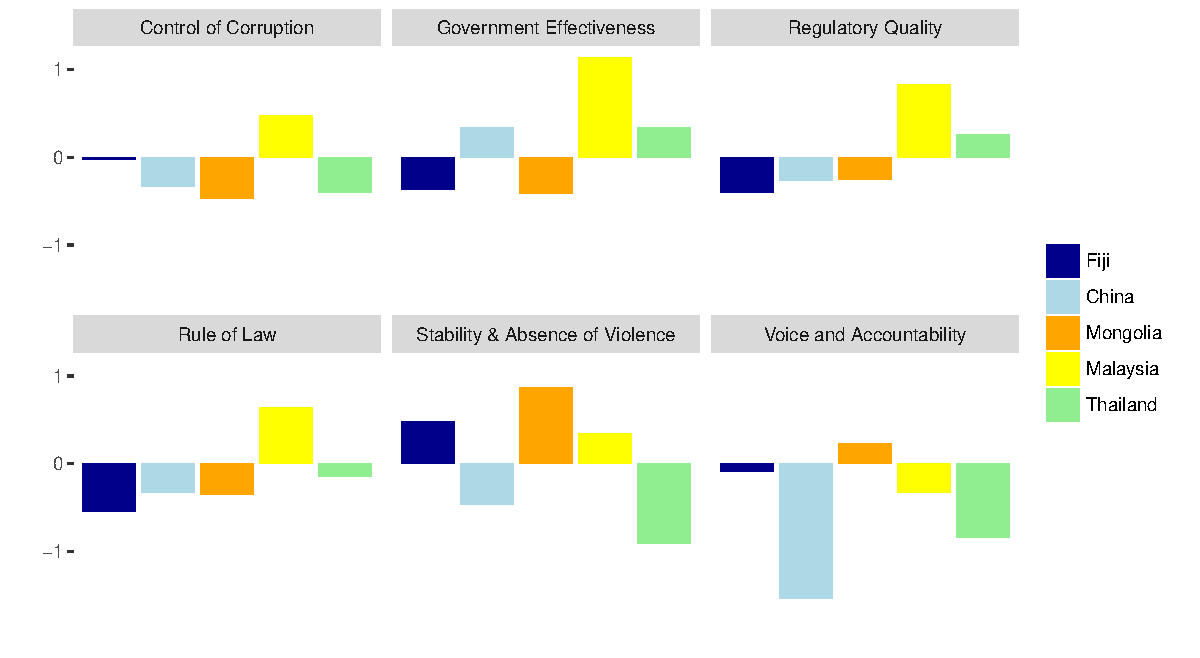
\includegraphics[width=\maxwidth]{figure/WGIindicators-1} 

}



    \vspace*{-0.6cm} 
    \hspace*{0.3cm} \raggedright\footnotesize{\href{http://data.worldbank.org/data-catalog/worldwide-governance-indicators}{Source: Worldwide Governance Indicators}}
  \end{minipage}
  \begin{minipage}[c]{0.48\textwidth} % Trade Policy table
    \vspace*{0.4cm}
  %\begin{flushleft}
    {\color{blue!50!black} \textbf{Trade Policy}}
  %\end{flushleft} 
  %\vspace*{0.2cm}
    \\[20pt]
    \centering
    \resizebox{\textwidth}{!}{%
% latex table generated in R 3.2.2 by xtable 1.7-4 package
% Wed Feb 17 09:01:55 2016
{\Large
\begin{tabular}{lrrr}
  & 2010 & 2014 &  \\ 
  \hline
Applied Tariff (Incl. Prefers. and Trade-Weighted) & 8.1 & 7.7 &  \\ 
  Binding (\%) & 100 & 100.0 &  \\ 
  Dispersion (Standard Deviation) & 48.4 & 45.9 &  \\ 
  Import duties collected (\%, 2010-2012) \large{[1]} & --- & 2.2 &  \\ 
  MFN Tariff (Agriculture) & 15.6 & 14.7 &  \\ 
  MFN Tariff (Non-Agriculture) & 8.8 & 8.8 &  \\ 
  MFN Tariff (Simple Average) & 9.7 & 9.6 &  \\ 
  Services sectors with GATS commitments \large{[1]} & --- & 93.0 &  \\ 
  \end{tabular}
}

    }
    \\[20pt]
    %\hspace*{0.5cm} 
    \raggedright{\footnotesize{\href{http://wits.worldbank.org}{Sources: WITS}{, }\href{http://stat.wto.org/CountryProfile/WSDBCountryPFHome.aspx?Language=E}{[1] WTO Trade Profiles}}}
  \end{minipage}
\end{minipage}

\vspace{+8ex}
%\hspace*{0.2cm}\subsection*{\color{white!50!black}Private Sector's Views}
\hspace*{0.1cm} \raggedright{\color{white!50!black}\Large Private Sector's Views}

\vspace*{-0.2cm}
{\color{white!30!black}\noindent\makebox[\linewidth]{\rule{18cm}{0.2pt}}} % horiz line

\begin{minipage}[b]{0.99\textwidth}
\vspace*{+0.6cm}
  \begin{minipage}[c]{0.02\textwidth}
  \hspace*{+0.1cm}
  \end{minipage}
  \begin{minipage}[c]{0.97\textwidth} 
    \begin{flushleft}  
      {\color{blue!50!black} \textbf{Enterprise Survey 2013}}
    \end{flushleft}  
    \vspace*{-0.4cm}
    \centering
    \resizebox{\textwidth}{!}{%
% latex table generated in R 3.2.2 by xtable 1.7-4 package
% Wed Feb 17 09:01:55 2016
{\Large
\begin{tabular}{lrrrl}
  & East Asia and Pacific & China & All Countries &  \\ 
  \hline
Number of electrical outages in a typical month & 3.50 & 0.10 & 6.30 &  \\ 
  Percent of firms with a bank loan/line of credit & 35.00 & 25.30 & 34.30 &  \\ 
  Proportion of investment financed by banks (\%) & 12.80 & 4.50 & 14.30 &  \\ 
  Proportion of investment financed internally (\%) & 74.70 & 89.60 & 71.80 &  \\ 
  Senior management time spent dealing with the requirements of government regulation (\%) & 6.70 & 0.90 & 9.90 &  \\ 
  \end{tabular}
}

    }
    \\[8pt]
    %\hspace*{0.3cm} 
    \raggedright{\footnotesize{\href{https://www.enterprisesurveys.org/data}{Source: Enterprise Survey 2013}}}
  \end{minipage} 

  \begin{minipage}[b]{0.99\textwidth} 
    \vspace{+4ex}
    \begin{minipage}[c]{0.49\textwidth} % top 5 constraints ES
      \center{\color{blue!50!black} \textbf{Top 5 constraints according to ES 2013 \\ \footnotesize(\% respondants)}}


{\centering 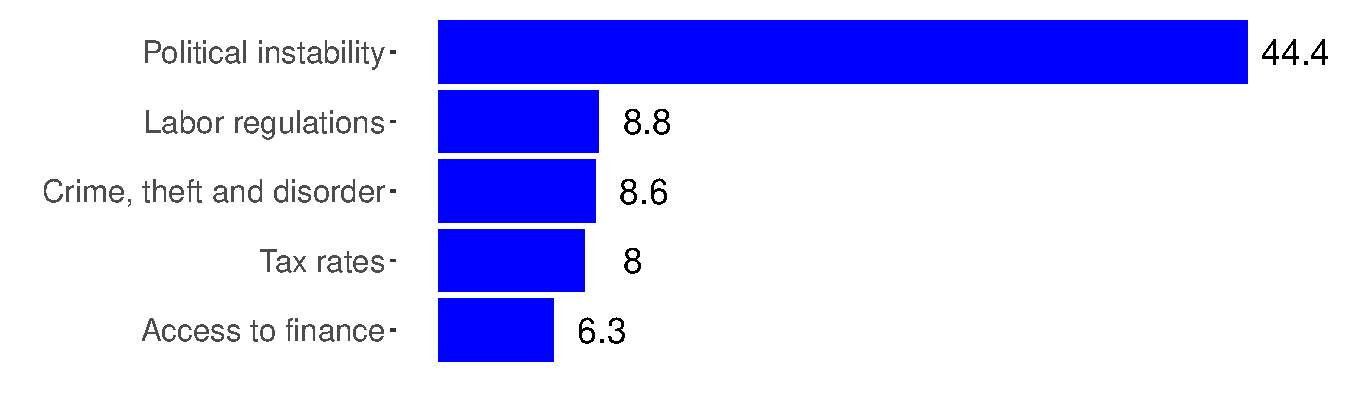
\includegraphics[width=\maxwidth]{figure/top5constraintsES-1} 

}



      %\vspace*{-0.7cm}
      \hspace*{0.3cm} \raggedright\footnotesize{\href{https://www.enterprisesurveys.org/data}{Source: Enterprise Survey 2013}}
    \end{minipage}
    \begin{minipage}[c]{0.49\textwidth} % top 5 constraints WEF
      \center{\color{blue!50!black} \textbf{Top 5 constraints according to WEF 2015 survey \\ \footnotesize(\% respondants among 88 executives)}}


{\centering 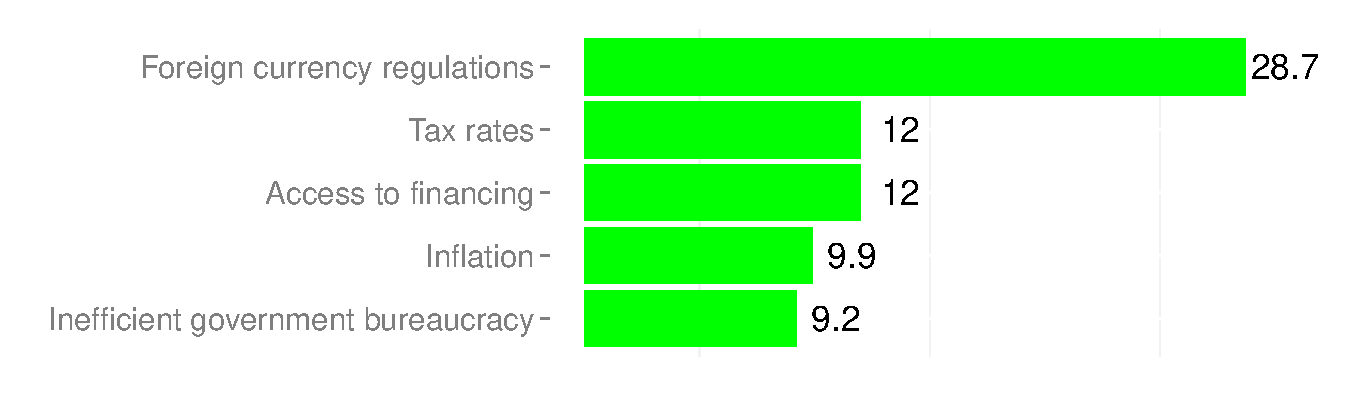
\includegraphics[width=\maxwidth]{figure/top5constraintsWEF-1} 

}



    %\vspace*{-0.7cm}
    \hspace*{0.3cm} \raggedright\footnotesize{\href{http://www.weforum.org/reports/global-competitiveness-report-2015-2016}{Source: WEF Global Competitiveness Report 2015}}
    \end{minipage}
  \end{minipage}
\end{minipage}

% \vspace{+8ex}
% {\color{blue!50!white}\noindent\makebox[\linewidth]{\rule{18cm}{0.3pt}}} % horiz line

% \vspace{+2ex}
% \begin{minipage}[c]{0.33\textwidth}
%   \hspace*{+0.3cm} \includegraphics[width=4cm,left]{/Users/asanchez3/shinyTCMN/www/wb_logo.jpg}
%   %\hspace*{+0.3cm} \includegraphics[width=4cm,left]{/Users/asanchez3/shinyTCMN/www/wb_logo.png}
% \end{minipage}
% \begin{minipage}[c]{0.65\textwidth}
%   \vspace*{-0.4cm}
%   \raggedleft{\color{white!40!black} \footnotesize TRADE AND COMPETITIVENESS MONITORING NOTE - UPDATED} 
%   %month year}
% \end{minipage}

%%%%%%%%%%%%%%%%%%%%%%%%%%%%%%%%%%%
%%%%%% Operations section %%%%%%%%%
%%%%%%%%%%%%%%%%%%%%%%%%%%%%%%%%%%%
\newpage
%%%%%%%%%%%%%%%% PAGE 3 %%%%%%%%%%%%%%%%%%%

%World Bank logo and TCMN branding
\begin{figure}
  \vspace{-3ex} % move up this figure
  \hspace{-7ex} % move left this figure
  \includegraphics[width=5cm]{/Users/asanchez3/shinyTCMN/www/wb_logo_background.png}
\end{figure}
\begin{figure}
  \begin{minipage}[t]{0.99\textwidth} % top section
      \vspace{-30ex}
      \hspace{-2ex}
      \raggedright{\includegraphics[width=5.5cm,right]{/Users/asanchez3/shinyTCMN/www/TC_snapshots_operations.png}}
  \end{minipage}
\end{figure}
%
%%%% Macro Indicators
\begin{minipage}[t]{0.99\textwidth} % top section
  \vspace{-1.5cm}
  \begin{minipage}[c]{0.36\textwidth} 
    \begin{minipage}[c]{0.28\textwidth} % flag
      \includegraphics[width=1.2cm,height=1.2cm]{/Users/asanchez3/shinyTCMN/www/CN.png}
    \end{minipage}
    \begin{minipage}[c]{0.70\textwidth} % Country name
      \section*{\color{blue!40!black}China}
    \end{minipage}
  \end{minipage}
  \begin{minipage}[c]{0.63\textwidth}
  %  \begin{flushleft}  
  %    \center{\color{blue!20!black} \textbf{\Large T\&C Product Line Operations Board Approved On or After FY14}}
  %  \end{flushleft} 
  \end{minipage}  
\end{minipage} % end top section

%\begin{minipage}[b]{0.99\textwidth} % main body
  \raggedright{\color{white!30!blue} \textbf{\Large SCD/CPF}}
    \begin{minipage}[c]{0.99\textwidth}  
      \vspace*{0.2cm}
      \raggedright{\color{white!30!blue} \textbf{\large Most Recent}}
      \vspace*{0.3cm}
      
% latex table generated in R 3.2.2 by xtable 1.7-4 package
% Wed Feb 17 09:01:55 2016
\scalebox{0.85}{
\begin{tabular}{>{\raggedright}p{5in}ll}
 Product & Document Date &  \\ 
  \hline
China - Performance and learning review of the country partnership strategy & 2016-02-10 &  \\ 
  \end{tabular}
}

      \vspace*{0.5cm}
    \end{minipage}
    
    \begin{minipage}[c]{0.99\textwidth} % imports/exports
      \vspace*{0.2cm}
      \raggedright{\color{white!30!blue} \textbf{\large Planned}}
      \vspace*{0.3cm}
      
% latex table generated in R 3.2.2 by xtable 1.7-4 package
% Wed Feb 17 09:01:55 2016
\scalebox{0.85}{
\begin{tabular}{>{\raggedright}p{5in}lll}
 Product & Concept Review Date & Board Date &  \\ 
  \hline
FY13-FY16 CPS Performance and Learning R & 2014-03-27 & 2016-02-04 &  \\ 
  Systematic Country Diagnostic & 2015-06-09 & 2016-04-29 &  \\ 
  \end{tabular}
}

      \vspace*{0.5cm}
    \end{minipage}
%\end{minipage}
  
\vspace*{0.5cm}
\raggedright{\color{white!30!blue} \textbf{\Large WB Lending Pipeline}}
\begin{minipage}[b]{0.99\textwidth} % overview tables
  \begin{minipage}[c]{0.99\textwidth}  
    \vspace*{0.5cm}
% latex table generated in R 3.2.2 by xtable 1.7-4 package
% Wed Feb 17 09:01:55 2016
{\footnotesize
\scalebox{0.85}{
\begin{tabular}{l>{\raggedright}p{1in}>{\raggedright}p{1in}>{\raggedright}p{0.5in}>{\raggedright}p{0.5in}>{\raggedright}p{0.5in}>{\raggedright}p{0.6in}>{\raggedright}p{0.5in}>{\raggedright}p{0.5in}>{\raggedleft}p{0.5in}>{\raggedleft}p{0.5in}l}
 Project ID & Project Name & Team Leader & Approval Date & Lending Inst. Type & Begin Appraisal & Commitment (US\$M) & Latest Sort Overall Risk Rating & FY Expenses (US\$K) & Cum Expenses (US\$K) & FY Prob &  \\ 
  \hline
None &  &  &  &  &  &  &  &  &  &  &  \\ 
  \end{tabular}
}
}

    \vspace*{0.5cm}
  \end{minipage}
    
  \raggedright{\color{white!30!blue} \textbf{\Large WB Portfolio}}
  \begin{minipage}[c]{0.99\textwidth} % imports/exports
    \vspace*{0.2cm}
    \raggedright{\color{white!30!blue} \textbf{\large Active}}
    \vspace*{0.3cm}
      
% latex table generated in R 3.2.2 by xtable 1.7-4 package
% Wed Feb 17 09:01:55 2016
{\footnotesize
\scalebox{0.85}{
\begin{tabular}{l>{\raggedright}p{1in}>{\raggedright}p{1in}>{\raggedright}p{0.5in}>{\raggedright}p{0.5in}>{\raggedright}p{0.5in}>{\raggedleft}p{0.5in}>{\raggedleft}p{0.5in}>{\raggedright}p{0.4in}>{\raggedright}p{0.4in}>{\raggedright}p{0.4in}>{\raggedleft}p{0.4in}l}
 Project ID & Project Name & Team Leader & Approval Date & Lending Inst. Type & Closing Date & Commitment (US\$M) & Undisbursed Balance (US\$M) & Project Rating DO & Project Rating IP & Overall Risk & Months in Problem Status &  \\ 
  \hline
None &  &  &  &  &  &  &  &  &  &  &  &  \\ 
  \end{tabular}
}
}

    \vspace*{0.5cm}
  \end{minipage}
     
  \begin{minipage}[c]{0.99\textwidth} % imports/exports 
    \raggedright{\color{white!30!blue} \textbf{\large Closed}}
    \vspace*{0.5cm}
      
% latex table generated in R 3.2.2 by xtable 1.7-4 package
% Wed Feb 17 09:01:56 2016
{\footnotesize
\scalebox{0.85}{
\begin{tabular}{l>{\raggedright}p{1.5in}>{\raggedright}p{1in}>{\raggedright}p{0.5in}>{\raggedright}p{0.5in}>{\raggedright}p{0.5in}>{\raggedleft}p{0.6in}>{\raggedright}p{0.5in}>{\raggedright}p{0.5in}>{\raggedright}p{0.5in}l}
 Project ID & Project Name & Team Leader & Approval Date & Lending Inst. Type & Closing Date & Commitment (US\$M) & Project Rating DO & Project Rating IP & IEG Outcome Rating &  \\ 
  \hline
None &  &  &  &  &  &  &  &  &  &  \\ 
  \end{tabular}
}
}

    \vspace*{0.5cm}
  \end{minipage}
     
\end{minipage}
 
 \newpage
%%%%%%%%%%%%%%%% PAGE 2 %%%%%%%%%%%%%%%%%%%
\begin{minipage}[t]{0.99\textwidth}
  \raggedright{\color{white!30!blue} \textbf{\Large WB ASA}}

  \begin{minipage}[b]{0.99\textwidth}
    \vspace*{0.2cm}
    \raggedright{\color{white!30!blue} \textbf{\large Active}}
    \vspace*{0.3cm}
  
% latex table generated in R 3.2.2 by xtable 1.7-4 package
% Wed Feb 17 09:01:56 2016
{\footnotesize
\scalebox{0.85}{
\begin{tabular}{l>{\raggedright}p{1in}>{\raggedright}p{1in}>{\raggedright}p{0.6in}>{\raggedright}p{0.6in}>{\raggedright}p{0.6in}>{\raggedleft}p{0.6in}>{\raggedleft}p{0.6in}>{\raggedleft}p{0.6in}>{\raggedleft}p{0.6in}l}
 Task ID & Task Name & Team Leader & Management Approval Date & Product Line & RAS (Y/N) & Current Expenditure BB (US\$K) & Current Expenditure Total (US\$K) & Lifetime Expenditure BB (US\$K) & Lifetime Expenditure Total (US\$K) &  \\ 
  \hline
P158921 & China SOE Reform & Chunlin Zhang & 2017-06-30 & TA & N & --- & 0 & --- & 0 &  \\ 
  \end{tabular}
}
}

     \vspace*{0.2cm}
  \end{minipage}

  \begin{minipage}[b]{0.99\textwidth}
    \vspace*{0.2cm}
    \raggedright{\color{white!30!blue} \textbf{\large Closed}}
    \vspace*{0.3cm}
       
% latex table generated in R 3.2.2 by xtable 1.7-4 package
% Wed Feb 17 09:01:56 2016
{\scriptsize
\scalebox{0.85}{
\begin{tabular}{l>{\raggedright}p{1in}>{\raggedright}p{1in}>{\raggedright}p{0.6in}>{\raggedright}p{0.6in}>{\raggedright}p{0.6in}>{\raggedleft}p{0.6in}>{\raggedleft}p{0.6in}>{\raggedleft}p{0.6in}>{\raggedleft}p{0.6in}l}
 Task ID & Task Name & Team Leader & Management Approval Date & Product Line & RAS (Y/N) & Current Expenditure BB (US\$K) & Current Expenditure Total (US\$K) & Lifetime Expenditure BB (US\$K) & Lifetime Expenditure Total (US\$K) &  \\ 
  \hline
P117571 & CN - Competition Policy & Hamid R. Alavi & 2010-06-28 & TA & N & --- & 0 &  65 &  65 &  \\ 
  P115366 & China in Regional Trade Agreements & Min Zhao & 2009-06-25 & EW & N & --- & 0 & 121 & 121 &  \\ 
  P112027 & PPIAF-SNTA:(CHI---) UDIC Credit Ratings & Kamran M. Khan & 2009-06-15 & PT & N & --- & 0 &  --- & 342 &  \\ 
  P107340 & China: Post-WTO Capacity Enhancement & Yan Wang & 2007-10-12 & TE & N & --- & 0 &  28 &  28 &  \\ 
  P103062 & China DL III: Ag  trade and poverty & Yan Wang & 2007-03-22 & TE & N & --- & 0 &  18 &  23 &  \\ 
  P104772 & China Agricultural Trade and Poverty & Yan Wang & 2007-03-20 & TE & N & --- & 0 &  20 &  23 &  \\ 
  P101477 & China GDLN Course: Agricultural Trade an & Yan Wang & 2006-11-16 & TE & N & --- & 0 &  22 &  22 &  \\ 
  P101478 & China DL I: Trade in Services & Yan Wang & 2006-10-12 & TE & N & --- & 0 &  28 &  28 &  \\ 
  P096748 & China: Trade and Poverty GDLN\# II & Yan Wang & 2005-10-27 & TE & N & --- & 0 &   9 &  10 &  \\ 
  P098085 & China: Trade in Services GDLN \# I & Yan Wang & 2005-09-29 & TE & N & --- & 0 &   8 &  10 &  \\ 
  P094096 & China: Trade in Services II & Yan Wang & 2005-06-09 & TE & N & --- & 0 &  --- &  22 &  \\ 
  P089375 & CHN-Trade in Services I & Yan Wang & 2005-03-31 & TE & N & --- & 0 &   7 &  20 &  \\ 
  P094445 & China's Participation in the WTO & Carsten Fink & 2005-02-22 & TE & N & --- & 0 &   1 &   1 &  \\ 
  P089372 & CHN-Trade and Support for the rural poor & Yan Wang & 2004-09-24 & TE & N & --- & 0 &  17 &  33 &  \\ 
  P092056 & CHN-Conference on trade policy & Yan Wang & 2004-09-10 & TE & N & --- & 0 &   9 &   9 &  \\ 
  \end{tabular}
}
}

    \vspace*{0.5cm}
  \end{minipage}

  \raggedright{\color{white!30!blue} \textbf{\Large IFC ASA}}
  \begin{minipage}[b]{0.99\textwidth}
    \vspace*{0.2cm}
    \raggedright{\color{white!30!blue} \textbf{\large Active}}
    \vspace*{0.3cm}
  
% latex table generated in R 3.2.2 by xtable 1.7-4 package
% Wed Feb 17 09:01:56 2016
{\scriptsize
\scalebox{0.85}{
\begin{tabular}{l>{\raggedright}p{1.6in}>{\raggedright}p{1.5in}>{\raggedright}p{0.7in}>{\raggedright}p{0.7in}>{\raggedleft}p{0.7in}>{\raggedleft}p{0.7in}>{\raggedleft}p{0.7in}l}
 Project ID & Project Name & Team Leader & IP Approval Date & Expected End Date & Approval Value (in US\$K) & Total Expenditures (in US\$K) & Current FY Expenditure (in US\$K) &  \\ 
  \hline
599555 & Green Building Regulation China Project & Sayyed, Autif Mohammed & 2013-07-31 & 2017-06-30 & 2,241 & 920 & 183 &  \\ 
  \end{tabular}
}
}

    \vspace*{0.2cm}
  \end{minipage}

  \raggedright{\color{white!30!blue} \textbf{\large Pipeline}}
  \vspace*{0.3cm}
  
% latex table generated in R 3.2.2 by xtable 1.7-4 package
% Wed Feb 17 09:01:56 2016
{\footnotesize
\scalebox{0.85}{
\begin{tabular}{l>{\raggedright}p{1.6in}>{\raggedright}p{1.5in}>{\raggedright}p{0.7in}>{\raggedright}p{0.7in}>{\raggedleft}p{0.7in}>{\raggedleft}p{0.7in}>{\raggedleft}p{0.7in}l}
 Project ID & Project Name & Team Leader & IP Approval Date & Expected End Date & Approval Value (in US\$K) & Total Expenditures (in US\$K) & Current FY Expenditure (in US\$K) &  \\ 
  \hline
None &  &  &  &  &  &  &  &  \\ 
  \end{tabular}
}
}

  \vspace*{0.2cm}
\end{minipage}

\begin{minipage}[b]{0.99\textwidth}
  \raggedright{\color{white!30!blue} \textbf{\large Closed}}
  \vspace*{0.3cm}
  
% latex table generated in R 3.2.2 by xtable 1.7-4 package
% Wed Feb 17 09:01:56 2016
{\scriptsize
\scalebox{0.85}{
\begin{tabular}{l>{\raggedright}p{1.6in}>{\raggedright}p{1.5in}>{\raggedright}p{0.7in}>{\raggedright}p{0.7in}>{\raggedleft}p{0.7in}>{\raggedleft}p{0.7in}>{\raggedleft}p{0.7in}l}
 Project ID & Project Name & Team Leader & IP Approval Date & Expected End Date & Approval Value (in US\$K) & Total Expenditures (in US\$K) & Current FY Expenditure (in US\$K) &  \\ 
  \hline
566267 & Sichuan Recovery Investment Promotion Component & Gu, Kuang Shen & 2008-10-16 & 2009-06-30 & 136 & 114 & 0 &  \\ 
  552007 & China Subnatl DB & Wang, Lihong & 2007-03-07 & 2008-09-30 & 252 & 243 & 0 &  \\ 
  530723 & Market and Structural Analysis of the Cement Sector in China & Gopalan, Prasad & 2006-09-25 & --- &   0 &   0 & 0 &  \\ 
  545504 & Tourism Development in Sichuan: A Value Chain Approach & Sun, Xiaolun & 2006-06-12 & 2007-12-31 & 248 & 233 & 0 &  \\ 
  540303 & Sichuan Cluster Development & Huang, Lin & 2006-04-02 & 2008-12-30 & 135 & 115 & 0 &  \\ 
  543984 & MOFCOM - China. IP-Support for lesser-developed regions. & Gu, Kuang Shen & 2006-02-13 & 2010-12-31 & 570 & 548 & 0 &  \\ 
  541484 & Sichuan Value Chain Analysis - CPDF/FIAS/SME Dept. joint project & Shen, Xiaofang & 2005-12-19 & 2007-07-31 & 310 & 233 & 0 &  \\ 
  538721 & Liaoning Administrative Barriers & Sun, Xiaolun & 2005-08-29 & --- &   0 &   0 & 0 &  \\ 
  538544 & Review of National Investment Promotion Policy & Battat, Joseph Y. & 2005-08-18 & --- &   0 &   0 & 0 &  \\ 
  538508 & Liaoning-Diagnostic Study & Battat, Joseph Y. & 2005-08-11 & --- &   0 &   0 & 0 &  \\ 
  521956 & Capacity Building of SIPB & Huang, Lin & 2005-06-20 & 2008-06-30 & 285 & 279 & 0 &  \\ 
  \end{tabular}
}
}

  \vspace*{0.2cm}
\end{minipage}
%%%%%%%%%%%%%%%% END OF DOCUMENT %%%%%%%%%%%%%%%%%%%
\end{document}
